\section{Results}

\subsection{Multihead $\mathDeePWAK$ learns sparse representations}

Multihead \DeePWAK learns remarkably sparse features (Fig. \ref{fig:blockE}) and clusters (Fig. \ref{fig:blockK}). 
Even more remarkably, all but one head appear bisemantic.
This is suggestive that the model may in fact be learning a tree structure to split the data along major features. These major features effectively split experimenter-labeled phenotypes (Fig. \ref{fig:hyper}). 

All of the more nuanced discrimination happens in \textsf{Head1}.
It splits the data into almost but not quite the maximum number of clusters, indicating our choice of $k$ is close to the latent concept space for (this projection of) the data.
Fascinatingly, the embeddings are even sparcer.

It should be empasized how surprising it is to see this much structure emerge from this data set. Contrast Fig. \ref{fig:params}. 1853 embryo halves is nothing by machine learning standards.
Though the data represent rich 3D microscopy images, these images were very crudely summarized by extracting 114 ad hoc statistics with no consideration for redundancy or significance.

\begin{figure}
  %\begin{subfigure}[b]{0.5\textwidth}
  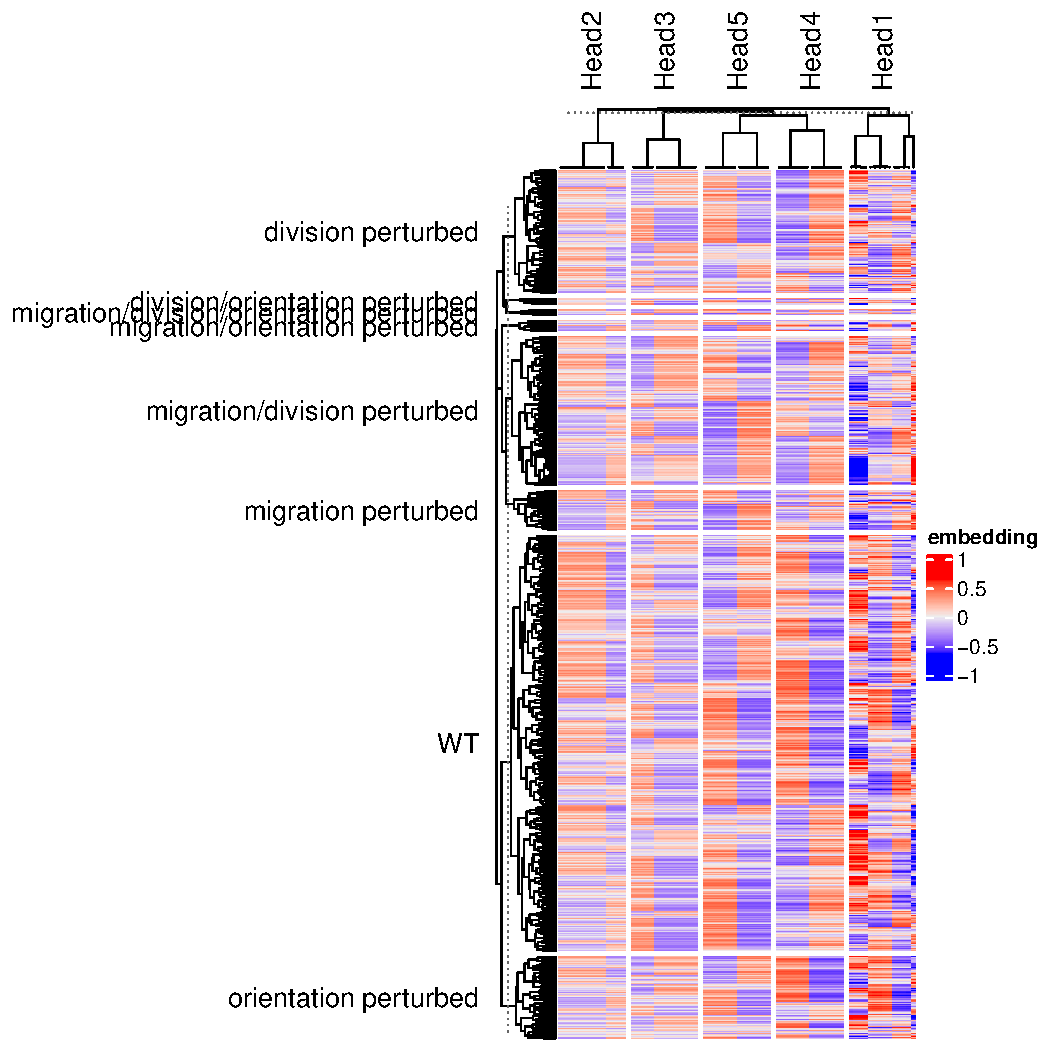
\includegraphics[width=\textwidth]{embeddings.pdf}
    \caption{DeePWAK learns sparse embedding values. }
    \label{fig:blockE}
\end{figure}

    
\begin{figure}
  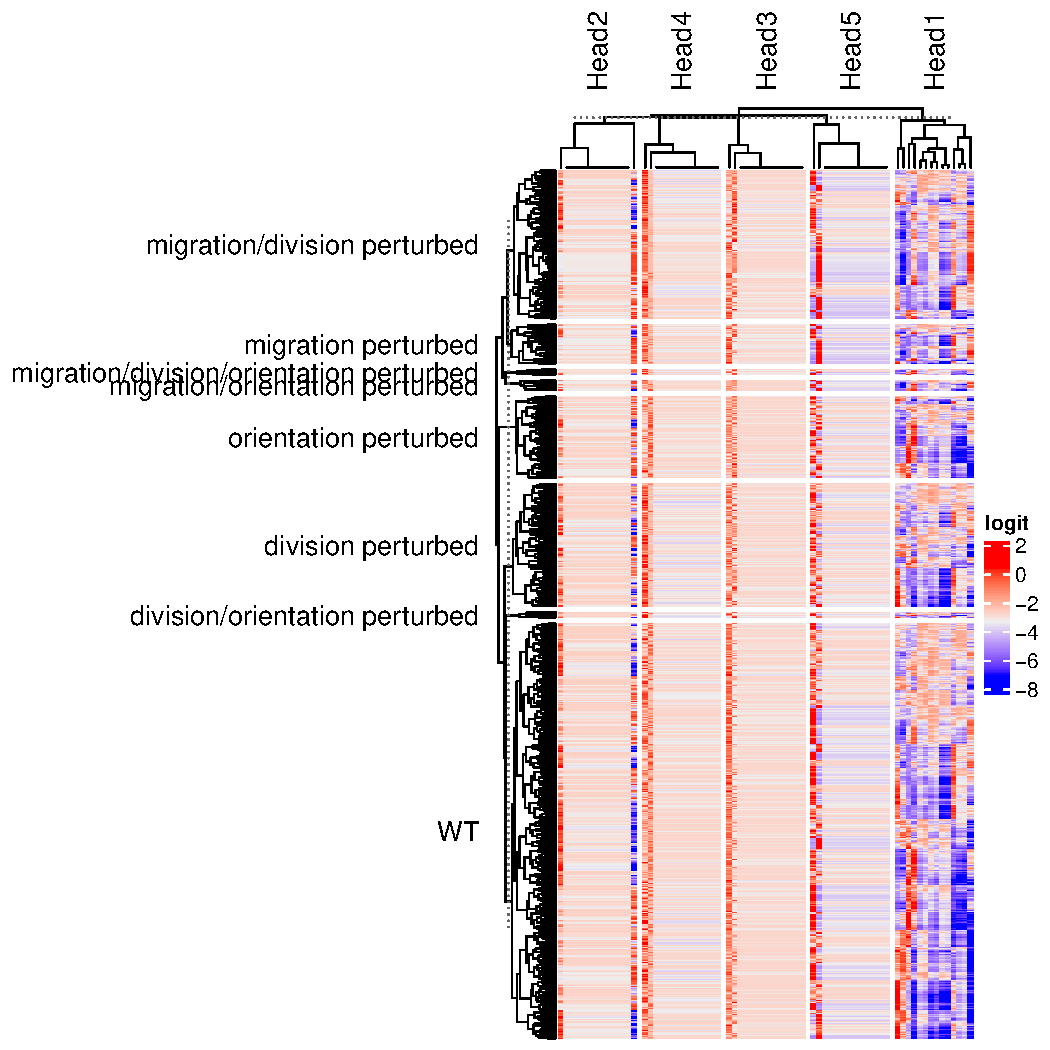
\includegraphics[width=\textwidth]{logits.pdf}
  \caption{For most heads, two clusters dominate.}
  \label{fig:blockK}
\end{figure}

\begin{figure}
  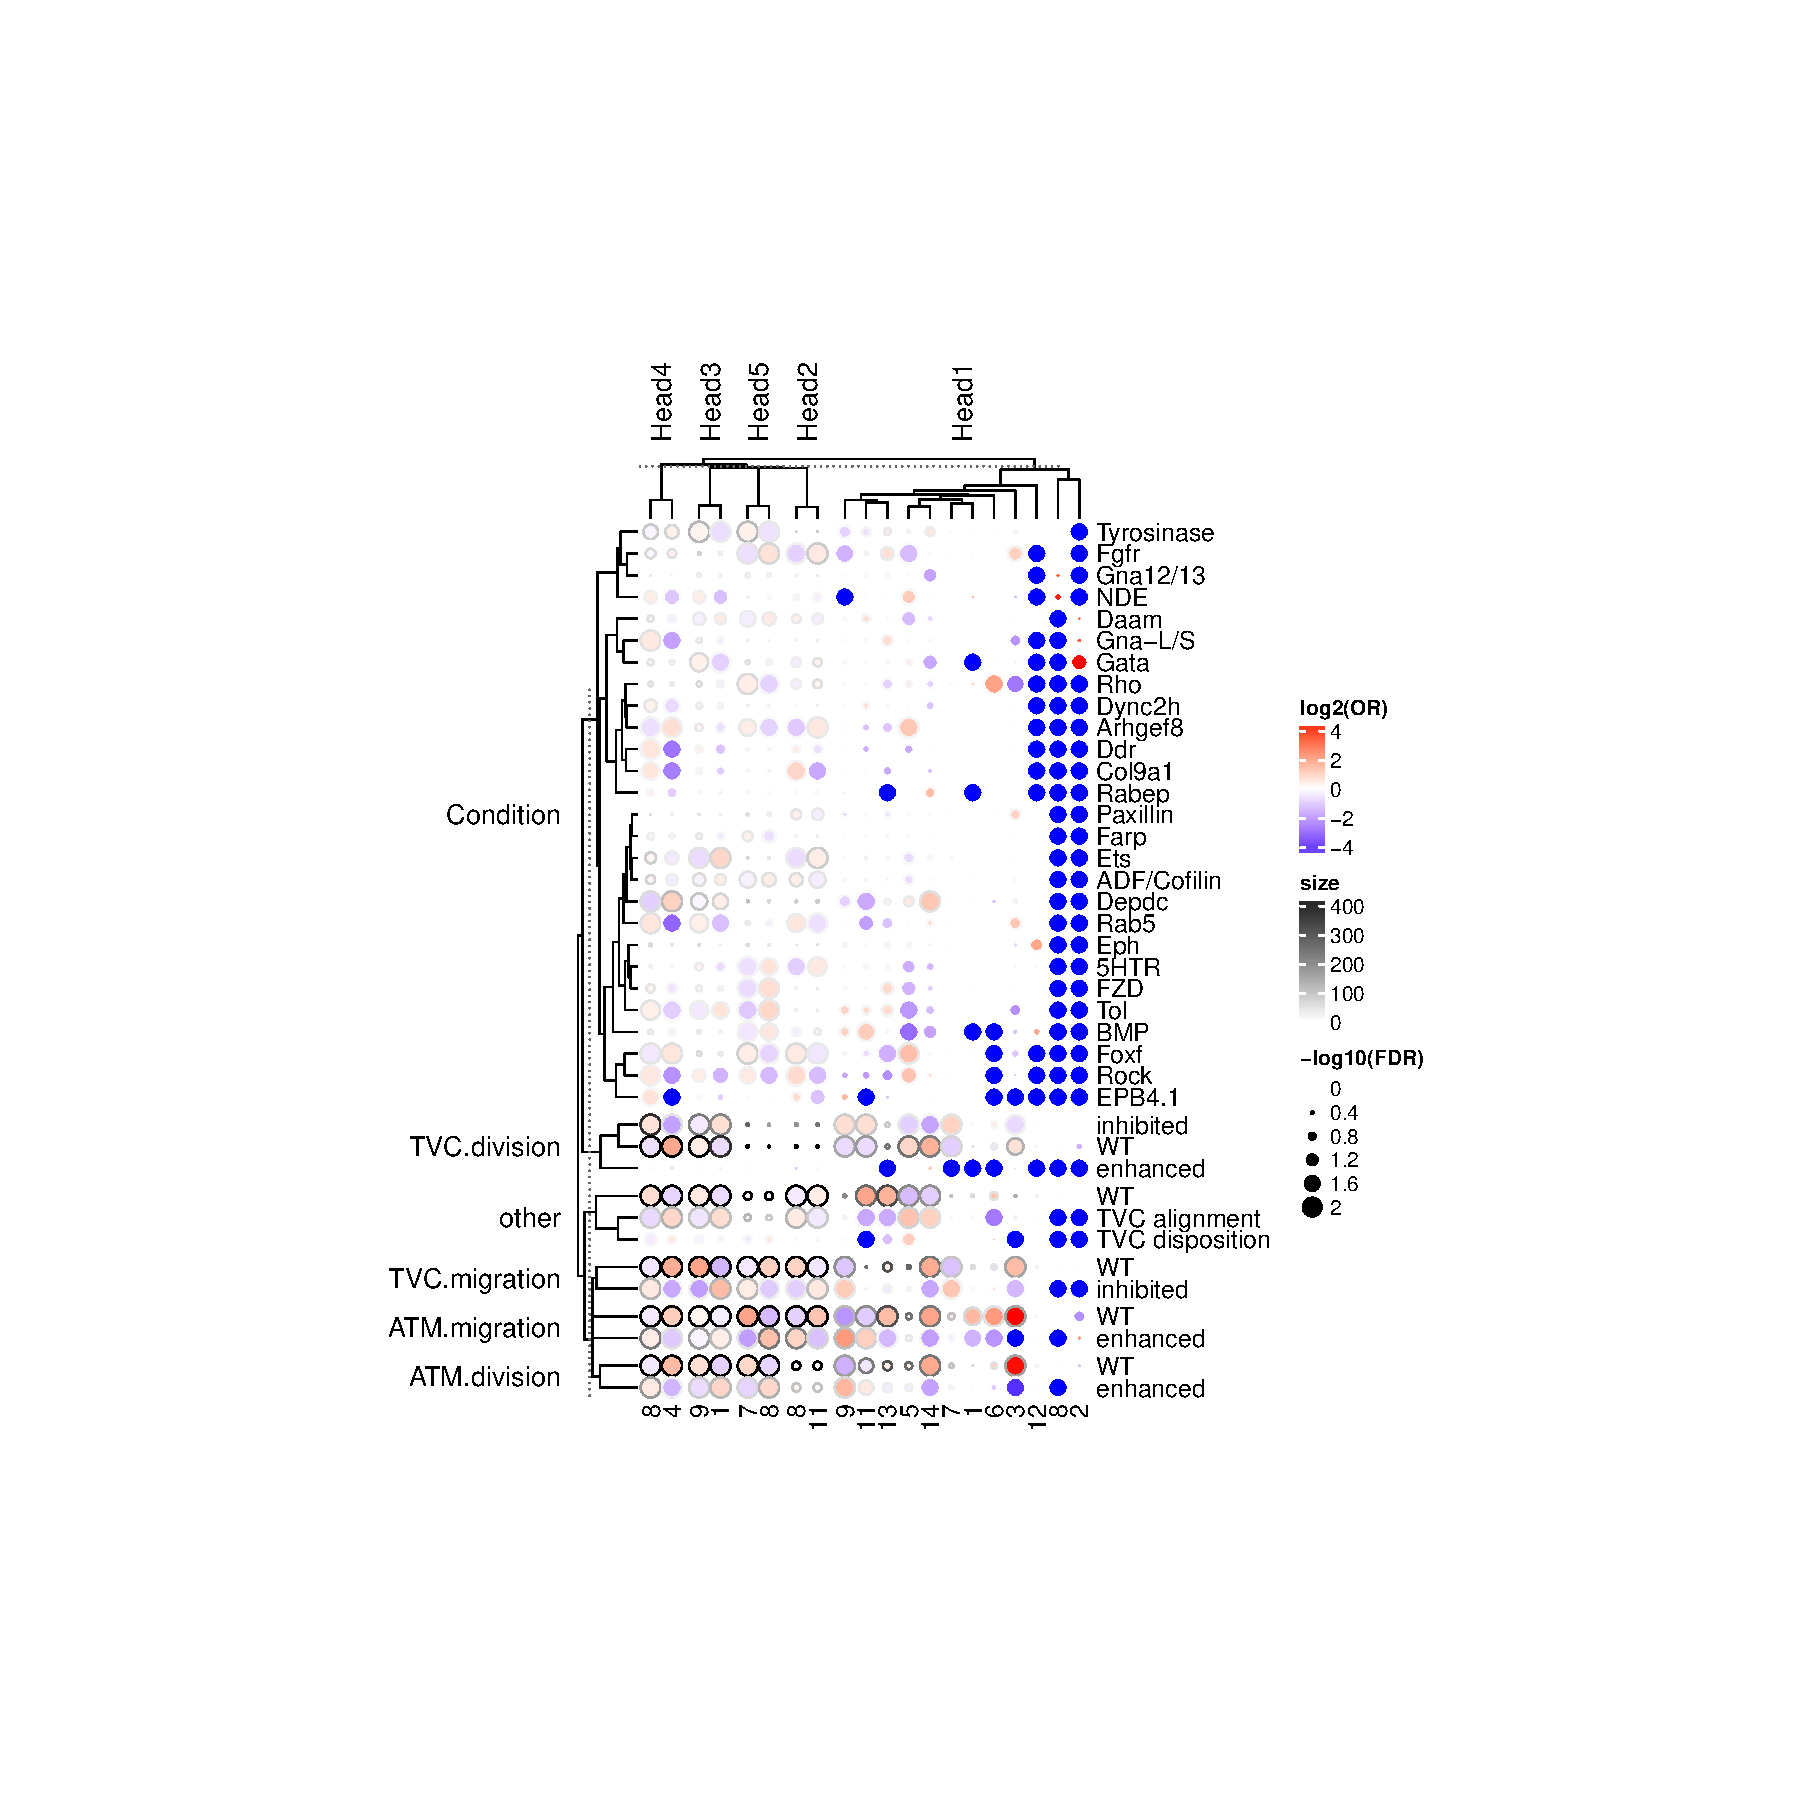
\includegraphics[width=\textwidth]{phenotype.pdf}
  \caption{Hypergeometric test for enrichment of phenotype and treatment condition for each cluster in each head. Dot color indicates overrepresentation of each category in a cluster compared to a uniform prior. Dot size indicates statistical significance of the difference. Dot outline shade indicates number of embryos represented by a dot. Head 1 appears ``polysemantic''. The others appear to distinguish single phenotypic categories.}
  \label{fig:hyper}
\end{figure}
